%%%%%%%%%%%%%%%%%%%%%%%%%%%%%%%%%%%%%%%%%%%%%%%%%%%%%%%%%%%%%%%%%%%%%%%%%%%%%%%%
%               CHAPTER 3: SYSTEM DESIGN & SECURITY ARCHITECTURE               %
%%%%%%%%%%%%%%%%%%%%%%%%%%%%%%%%%%%%%%%%%%%%%%%%%%%%%%%%%%%%%%%%%%%%%%%%%%%%%%%%

\chapter{System Design and Security Architecture}\label{section:architecture}

%%%%%%%%%%%%%%%%%%%%%%%%%%%%%%%%%%%%%%%%%%%%%%%%%%%%%%%%%%%%%%%%%%%%%%%%%%%%%%%%
%           SECTION 3.1: ARCHITECTURAL OVERVIEW & SERVICE ORGANIZATION         %
%%%%%%%%%%%%%%%%%%%%%%%%%%%%%%%%%%%%%%%%%%%%%%%%%%%%%%%%%%%%%%%%%%%%%%%%%%%%%%%%

\section{Architectural Overview and Service Organization}\label{section:arch-overview}

\textit{CryptoShred Health} runs as an isolated, multi-tier microservice cluster engineered to enforce zero-plaintext storage across all backend databases while serving real-time clinical workflows. The platform is divided into seven operational layers:
\begin{enumerate}
    \item \textbf{Presentation Layer (React 19):} A fast, modern React single-page web dashboard built with Vite and providing role-based dashboards for clinicians and auditors, providing patient intake, clinical visit records, lifecycle status toggles, and client-side cryptographic Merkle proof verification.
    \item \textbf{Application Core (Spring Boot 3.3.4):} A stateless Java~21 backend managing JWT authentication, transactional database operations, HashiCorp Vault KMS interactions, and asynchronous Kafka audit publishing.
    \item \textbf{Key Management Tier (3-Node Vault Raft Cluster):} A high-availability KMS behind an HAProxy load balancer, exposing the Transit Engine for two-tier envelope key wrapping, cryptographic key destruction, and classical RSA-2048 signing as part of the platform's hybrid post-quantum deletion proof engine.
    \item \textbf{Persistence Tier (PostgreSQL 15):} Relational storage where all demographic and clinical fields persist strictly as AES-256-GCM ciphertexts, ensuring zero plaintext exists in database tables or write-ahead logs.
    \item \textbf{Caching Tier (Redis 7 L2):} An in-memory cache holding decrypted patient records for 15 minutes, with an automatic filter that bypasses lookups for shredded records to eliminate database load.
    \item \textbf{Event Streaming (Kafka 3.7 KRaft):} An append-only broker recording nine entity lifecycle events across a 365-day immutable audit topic for regulatory provenance and historical replay.
    \item \textbf{Observability Stack (Prometheus \& Grafana):} Telemetry pipelines scraping JVM memory, connection pools, and Vault Transit latency histograms into unified operational dashboards.
\end{enumerate}

All microservices run inside Docker containers attached to an isolated internal bridge network. While the local development Compose configuration publishes container ports to the host for developer tooling and debugging, in production deployments, PostgreSQL, Vault, Redis, and Kafka bind exclusively to private container interfaces with zero public port exposure, while an Nginx edge gateway terminates external TLS~1.3 connections. 

Figure~\ref{fig:system-architecture} illustrates the system topology, component interactions, and network security boundaries across these seven tiers.

\begin{figure}[H]
    \centering
    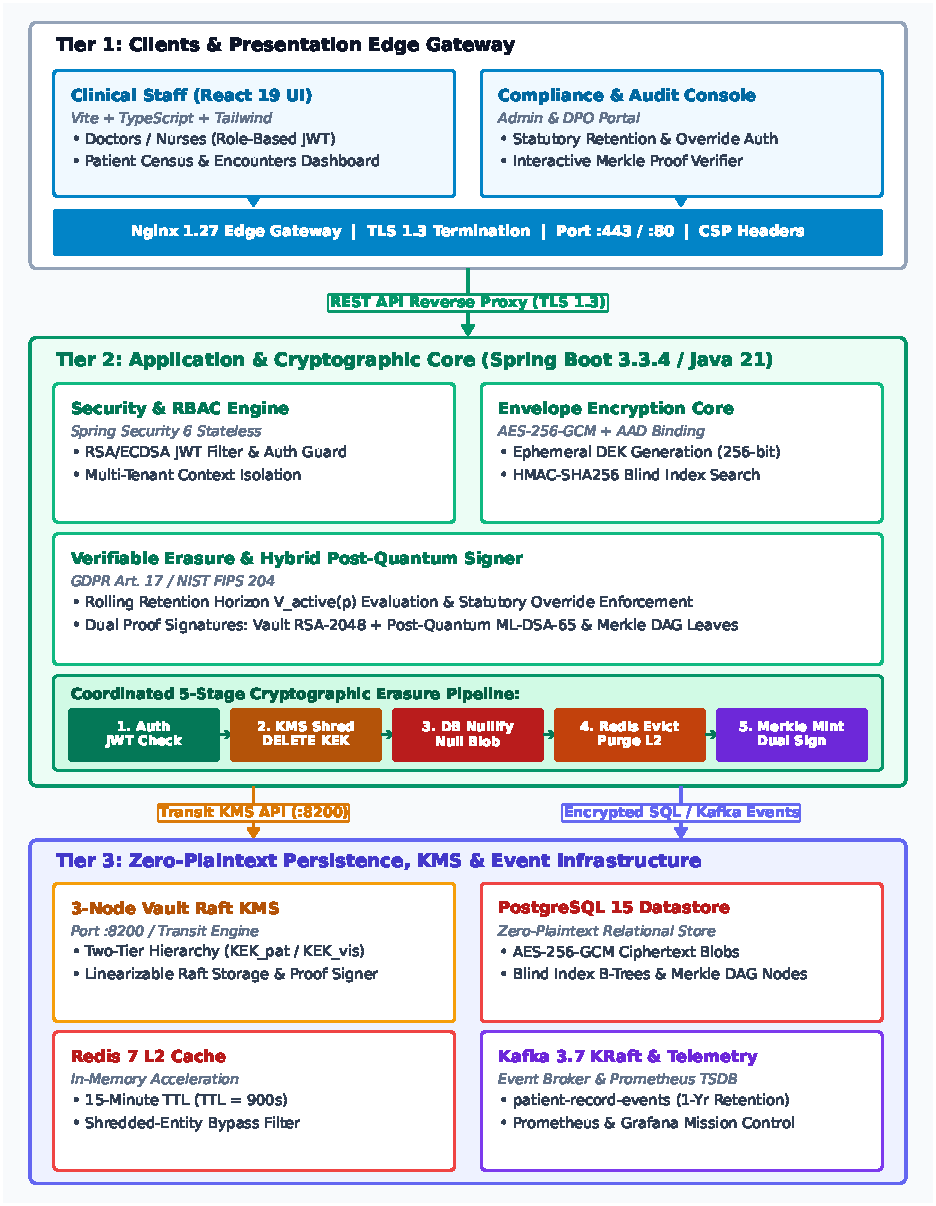
\includegraphics[width=\textwidth]{figures/fig_system_architecture.pdf}
    \caption{\textit{CryptoShred Health} multi-tier system architecture and network security boundaries.}
    \label{fig:system-architecture}
\end{figure}

\subsection{End-to-End System Workflows}

Data processing workflows enforce strict cryptographic boundaries at each transaction step:
\begin{itemize}
    \item \textbf{Patient Ingestion and Encryption Pipeline:} During patient registration, the frontend sends an authenticated JSON payload over TLS~1.3 to the backend API. The backend generates an ephemeral 256-bit AES Data Encryption Key (DEK), encrypts the demographic fields using AES-256-GCM, and dispatches the DEK to Vault Transit. Vault wraps the DEK under the patient's dedicated Key Encryption Key ($\text{KEK}_{\text{patient}}$) and returns the wrapped blob. The backend derives salted HMAC-SHA256 blind index tokens for searchable fields, commits the ciphertext and wrapped DEK to PostgreSQL within a single ACID transaction, and dispatches an audit event to Kafka.

    \item \textbf{Encrypted Record Retrieval Pipeline:} When a clinician requests a patient file, the backend queries the Redis L2 cache. On a cache hit, it returns the decrypted DTO immediately. On a cache miss, the backend reads the ciphertext blob and wrapped DEK from PostgreSQL, sends the wrapped DEK to Vault Transit for unwrapping, decrypts the payload in temporary heap memory using AES-256-GCM, writes the decrypted record to Redis with a 900-second TTL, wipes the raw DEK bytes, and returns the clinical plaintext.

    \item \textbf{Cryptographic Shredding Pipeline:} Upon receiving an authorized GDPR Article~17 erasure request, the backend instructs Vault Transit to delete the corresponding Key Encryption Key ($\text{KEK}_{\text{patient}}$ or $\text{KEK}_{\text{visit}}$). Because all historical database rows, write-ahead log records, Kafka topic segments, and offline backups hold ciphertexts tied to this KEK, destroying the key renders those payloads permanently unrecoverable. In live PostgreSQL storage, the backend sets \texttt{encrypted\_data\_blob = NULL}, clears blind index columns (\texttt{blind\_index\_nhs}, \texttt{blind\_index\_mrn}, \texttt{blind\_index\_last\_name} $\rightarrow$ \texttt{NULL}), sets \texttt{shredded = true} and \texttt{is\_active = false}, evicts Redis cache keys, emits a \texttt{PATIENT\_SHREDDED} event to Kafka, appends a deletion leaf into the Merkle DAG, and signs a dual-scheme deletion certificate.

    \item \textbf{Administrative Deactivation and Reactivation:} When a patient is discharged or placed on hold, clinical administrators invoke \texttt{PATCH /api/patients/\{id\}/deactivate}. The backend sets \texttt{is\_active = false}, purges Redis, and publishes a \texttt{PATIENT\_DEACTIVATED} event to Kafka while preserving the Vault KEK and encrypted database rows. When treatment resumes, \texttt{PATCH /api/patients/\{id\}/activate} flips \texttt{is\_active = true} and broadcasts a \texttt{PATIENT\_ACTIVATED} event.
\end{itemize}

%%%%%%%%%%%%%%%%%%%%%%%%%%%%%%%%%%%%%%%%%%%%%%%%%%%%%%%%%%%%%%%%%%%%%%%%%%%%%%%%
%     SECTION 3.2: DUAL-LEVEL ENVELOPE ENCRYPTION & BLIND INDEX ARCHITECTURE    %
%%%%%%%%%%%%%%%%%%%%%%%%%%%%%%%%%%%%%%%%%%%%%%%%%%%%%%%%%%%%%%%%%%%%%%%%%%%%%%%%

\section{Dual-Level Envelope Encryption and Blind Index Search Architecture}\label{section:encryption-indexing}

Using a single master key to encrypt an entire hospital database creates a dangerous single point of failure. If that key is compromised, every patient record in the facility is exposed at once. \textit{CryptoShred Health} eliminates this risk by assigning distinct keys to each patient profile and individual medical visit, binding ciphertexts directly to entity IDs, and using salted blind indexes for fast, secure lookups.

\subsection{Two-Tier Key Hierarchy and Ciphertext Packaging}

The platform isolates cryptographic access boundaries by maintaining separate keys for demographic identities and individual clinical visits:
\begin{enumerate}
    \item \textbf{Patient Demographic KEK ($\text{KEK}_{\text{patient}}$):} Provisioned in Vault Transit at \texttt{transit/keys/patient\_\{uuid\}}. This key protects demographic identifiers including patient names, birth dates, national identifiers, and home addresses.

    \item \textbf{Clinical Visit KEK ($\text{KEK}_{\text{visit}}$):} Provisioned at \texttt{transit/keys/patient\_\{uuid\}\_visit\_\{uuid\}}. Every distinct consultation, lab result, and diagnostic note receives an independent KEK.
\end{enumerate}

This key separation enables fine-grained data revocation while defining distinct algorithmic complexity classes for erasure:
\begin{itemize}
    \item \textbf{Demographic Identity Shredding ($\mathcal{O}(1)$):} Destroying the patient master key ($\text{KEK}_{\text{patient}}$) is a strict constant-time $\mathcal{O}(1)$ operation. A single Vault Transit API call permanently destroys $\text{KEK}_{\text{patient}}$, instantly collapsing all demographic identity attributes (names, birth dates, national identifiers, addresses) into computationally unrecoverable noise. This severs the cryptographic link between the individual and their historical records in $5.63\text{--}7.65\text{~ms}$, fulfilling GDPR Article~17 for demographic erasure regardless of the volume of past visits.
    \item \textbf{Complete Encounter Chart Erasure ($\mathcal{O}(m)$):} While destroying $\text{KEK}_{\text{patient}}$ anonymizes the clinical history, individual clinical encounters and diagnostic attachments remain encrypted under their respective encounter keys $\text{KEK}_{\text{visit}}$. To achieve total cryptographic eradication of a patient's entire medical chart containing $m$ historical visits, the system must execute $m$ independent key destruction operations in Vault Transit. This complete chart purge exhibits deterministic linear scaling $\mathcal{O}(m)$. Because each Vault key destruction executes with sub-$2\text{~ms}$ latency ($1.69\text{~ms}$ measured), purging a typical multi-visit chart ($m = 25$) completes in approximately $42.3\text{~ms}$, preserving interactive responsiveness without acquiring relational database table locks.
\end{itemize}

Unstructured binary attachments---such as clinical PDF documents, laboratory reports, and diagnostic imaging scans---anchor directly into this cryptographic hierarchy under the parent consultation's $\text{KEK}_{\text{visit}}$. Rather than storing raw files on unencrypted network file shares that risk orphaned data persistence after erasure, the platform encapsulates each file into a zero-plaintext binary record (\texttt{PatientAttachment}). Ephemeral 256-bit DEKs encrypt the raw file bytes via AES-256-GCM using unique 96-bit initialization vectors, after which the DEK is wrapped under the encounter's $\text{KEK}_{\text{visit}}$. The resulting Base64 ciphertext blob is stored directly in relational storage. When a clinical visit is crypto-shredded, all linked binary attachments undergo an automatic cryptographic cascade: live database ciphertext pointers and IVs are set to \texttt{NULL}, while historical backup snapshots containing the raw encrypted file bytes become permanently undecryptable because the parent $\text{KEK}_{\text{visit}}$ is permanently eradicated inside HashiCorp Vault.

When encrypting payloads, the backend serializes the Java DTO into JSON bytes, creates an ephemeral 256-bit $K_{\text{DEK}}$ via \texttt{SecureRandom}, and executes AES-256-GCM encryption with contextual Additional Authenticated Data (AAD) parameters:
\begin{equation}
    W_{\text{DEK}} = \text{Vault-Transit-Wrap}(K_{\text{KEK}}, K_{\text{DEK}})
    \label{eq:vault-wrap}
\end{equation}
In Equation~\ref{eq:vault-wrap}, Vault encrypts the ephemeral key under the persistent master key $K_{\text{KEK}}$ inside the KMS process. The application packages ciphertext $C$, 96-bit initialization vector, 128-bit authentication tag $T$, and wrapped key $W_{\text{DEK}}$ into a Base64-encoded JSON payload stored in PostgreSQL's \texttt{encrypted\_data\_blob} column. Once written to disk, the backend zeroes raw $K_{\text{DEK}}$ byte buffers in memory using \texttt{Arrays.fill(dek, (byte) 0)}.

\subsection{Cryptographic Context Binding via Additional Authenticated Data (AAD)}

To enforce the cryptographic context binding model established in Section~\ref{section:crypto-foundations} (Equation~\ref{eq:aes-gcm-formal}), the storage engine binds the AES-256-GCM authentication tag directly to public record identifiers through Additional Authenticated Data (AAD):
\begin{equation}
    \text{AAD} = \text{UTF-8}(\text{EntityID})
    \label{eq:aad-binding}
\end{equation}
In Equation~\ref{eq:aad-binding}, the $\text{AAD}$ string encodes the public business identifier (\texttt{patientId} for demographic profiles or \texttt{visitId} for clinical encounters) as UTF-8 bytes. During decryption, the cipher recalculates the 128-bit authentication tag against the expected entity UUID. If an adversary transposes a ciphertext payload between database records, tag verification fails immediately, causing the engine to abort with an \texttt{AEADBadTagException} prior to exposing clinical plaintext in application memory.

\subsection{Deterministic Blind Indexing for Exact-Match Search}

Applying the cryptographic foundation established in Section~\ref{section:crypto-foundations} (Equation~\ref{eq:blind-index-theory}), the platform maps each searchable attribute $f \in \{\text{NHS Number}, \text{MRN}, \text{Surname}\}$ to a dedicated 64-character hexadecimal column: \texttt{blind\_index\_nhs}, \texttt{blind\_index\_mrn}, and \texttt{blind\_index\_last\_name}. PostgreSQL maintains standard B-Tree indexes over these columns, avoiding full-table decryptions while preserving sub-millisecond point query execution via $\mathcal{O}(\log N)$ B-tree lookups.

When an authenticated clinician executes an exact-match query, the backend computes the deterministic blind index $B_{\text{search}} = \text{BlindIndex}(v_f)$ using the Vault-managed secret HMAC key $K_{\text{salt}}$ and executes the indexed filter directly against PostgreSQL:
\begin{equation}
    \text{SELECT * FROM patients WHERE blind\_index\_nhs} = B_{\text{search}}
    \label{eq:sql-blind-search}
\end{equation}

This relational construction enforces three operational security controls:
\begin{enumerate}
    \item \textbf{DBA Confidentiality:} Database administrators inspecting raw disk blocks or SQL dumps observe only pseudorandom HMAC hashes, preventing patient re-identification.
    \item \textbf{Rainbow Table Inversion Defense:} Because HMAC-SHA256 incorporates the 256-bit secret salt $K_{\text{salt}}$, precomputed rainbow tables and dictionary attacks cannot invert common surnames or formatted NHS identifiers.
    \item \textbf{Instant Lookup Revocation:} When an entity is shredded, the backend overwrites blind index columns with \texttt{NULL}, permanently disabling index scans across all future queries.
\end{enumerate}

%%%%%%%%%%%%%%%%%%%%%%%%%%%%%%%%%%%%%%%%%%%%%%%%%%%%%%%%%%%%%%%%%%%%%%%%%%%%%%%%
%        SECTION 3.3: VERIFIABLE DELETION & HYBRID SIGNING PROTOCOL            %
%%%%%%%%%%%%%%%%%%%%%%%%%%%%%%%%%%%%%%%%%%%%%%%%%%%%%%%%%%%%%%%%%%%%%%%%%%%%%%%%

\section{Verifiable Cryptographic Deletion and Hybrid Signing Protocol}\label{section:shredding-proofs}

Standard file and row deletions in distributed databases provide no cryptographic evidence of destruction. External auditors cannot confirm whether deleted records remain cached on replica nodes, write-ahead logs, or cold backup media. CryptoShred Health transforms erasure into an auditable cryptographic receipt validated by post-quantum signatures and Merkle inclusion proofs.

\subsection{The Five-Stage Cryptographic Erasure Pipeline}

When clinical staff or automated compliance engines trigger an erasure request, the backend coordinates a five-stage deletion sequence:
\begin{enumerate}
    \item \textbf{Stage 1: Authorization and Scope Determination:} The security filter verifies the caller's JWT claims, requiring \texttt{ADMIN} or \texttt{DOCTOR} privileges, and identifies whether the request targets an individual clinical encounter or the entire patient history.

    \item \textbf{Stage 2: KMS Master Key Destruction:} The backend issues a deletion request to the Vault Transit KMS:
    \begin{equation}
        \text{DELETE } /v1/\text{transit/keys/patient\_}\{uuid\}
        \label{eq:vault-delete}
    \end{equation}
    Vault zeroes the key material in memory and replicates key destruction across all Raft followers in $5.6\text{--}7.6\text{~ms}$. Without this key, all associated ciphertexts across database rows, write-ahead log records, Kafka topics, and backup tapes become irrecoverable.

    \item \textbf{Stage 3: PostgreSQL Nullification and Flagging:} Within the active transaction, the backend sets \texttt{encrypted\_data\_blob = NULL}, clears search columns (\texttt{blind\_index\_nhs = NULL}, \texttt{blind\_index\_mrn = NULL}, \texttt{blind\_index\_last\_name = NULL}), and sets \texttt{shredded = true} and \texttt{is\_active = false}, preventing search lookups while keeping non-PII audit timestamps for compliance tracking.

    \item \textbf{Stage 4: Cache Eviction and Event Emission:} The backend evicts cached entries from Redis and publishes a \texttt{PATIENT\_SHREDDED} or \texttt{VISIT\_SHREDDED} event to the Kafka \texttt{patient-record-events} topic, signaling downstream services to purge transient data.

    \item \textbf{Stage 5: Binary Merkle Tree Accumulation and Certificate Generation:} The platform records the deletion leaf into the append-only binary Merkle tree, calculates the updated root hash, and mints a dual-signed deletion certificate combining classical RSA PKCS\#1 v1.5 (\texttt{SHA256withRSA}) inside Vault and post-quantum CRYSTALS-Dilithium3 (standardized in NIST FIPS~204 as ML-DSA-65) in the backend.
\end{enumerate}

Figure~\ref{fig:erasure-sequence} illustrates the end-to-end execution sequence across the 5-stage cryptographic erasure pipeline.

\begin{figure}[htbp]
    \centering
    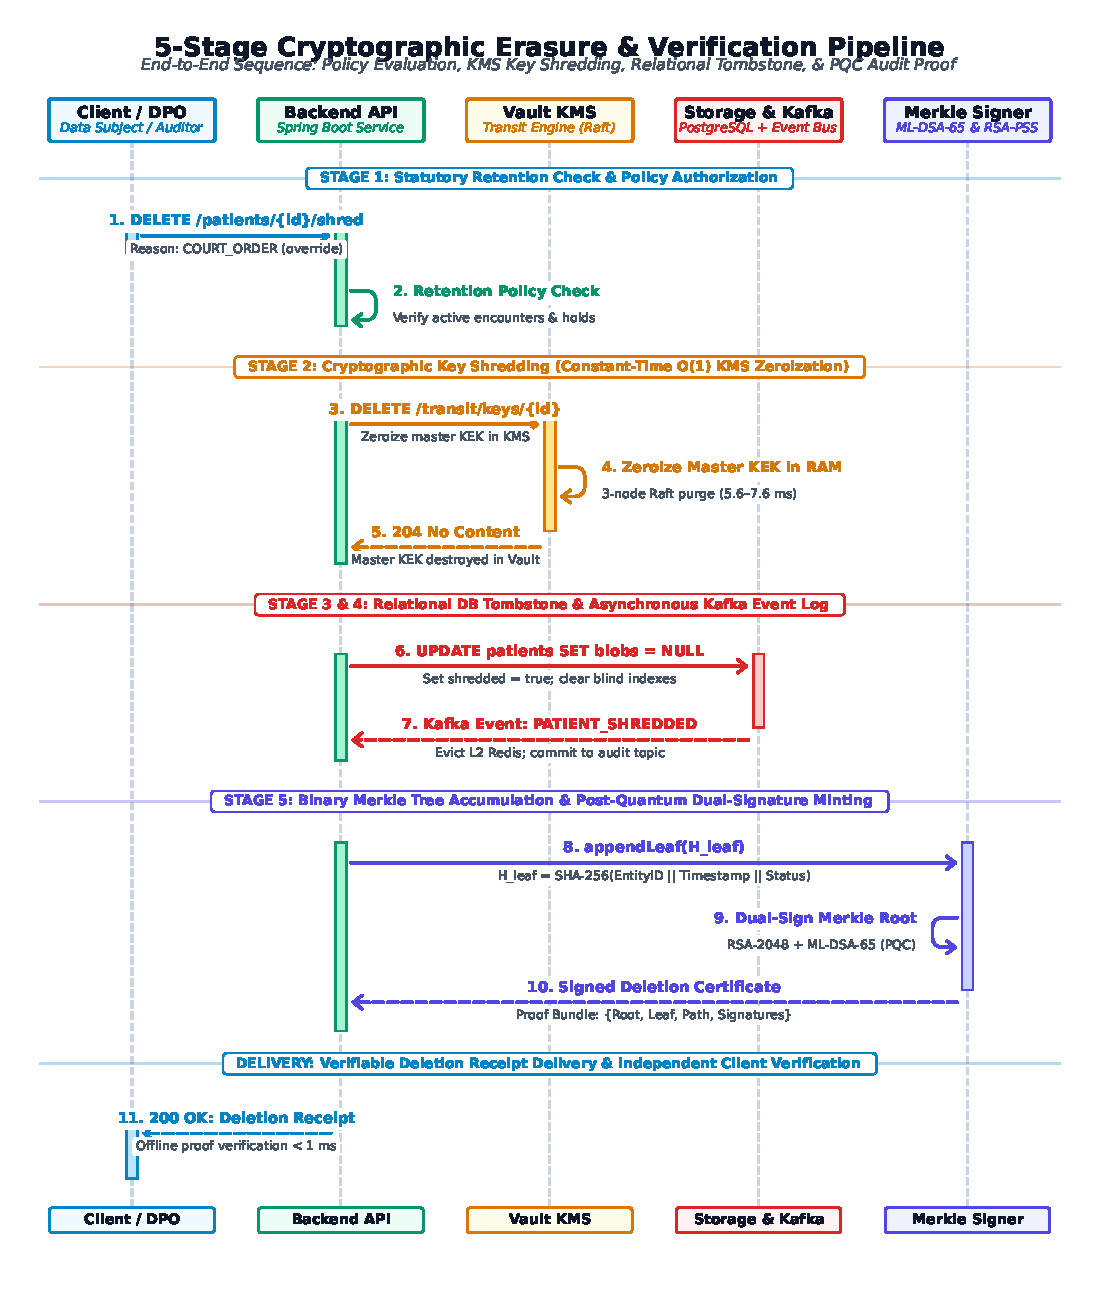
\includegraphics[width=\textwidth]{figures/fig_erasure_sequence.pdf}
    \caption{Sequence diagram illustrating the 5-stage cryptographic erasure pipeline across Client/DPO, Spring Boot backend, HashiCorp Vault Transit KMS, PostgreSQL, Redis, Kafka, and the Binary Merkle Tree. In Stage~5, deletion certificates are signed using classical RSA PKCS\#1 v1.5 (\texttt{SHA256withRSA}) via Vault Transit and post-quantum CRYSTALS-Dilithium3 (ML-DSA-65) via the backend signing service.}
    \label{fig:erasure-sequence}
\end{figure}

\subsection{Policy-Driven Rolling Retention Horizon and Active Encounter Dynamics}

Patients accumulate medical visits over decades, during which individual encounters may be deleted due to consent withdrawal or court orders. To balance GDPR Article~17 deletion requests with legal retention mandates like NHS and HIPAA, \textit{CryptoShred Health} implements a dynamic rolling retention horizon evaluated strictly across active, non-shredded encounters.

Let $p$ represent a patient registered at timestamp $t_{\text{registered}}(p)$, and let $\mathcal{V}(p) = \{v_1, v_2, \dots, v_m\}$ denote all linked medical visits. We define the active encounter set $\mathcal{V}_{\text{active}}(p)$ as:
\begin{equation}
    \mathcal{V}_{\text{active}}(p) = \left\{ v \in \mathcal{V}(p) \;\middle|\; \text{isShredded}(v) = \text{false} \right\}
    \label{eq:active-encounter-set}
\end{equation}
In Equation~\ref{eq:active-encounter-set}, $\mathcal{V}_{\text{active}}(p)$ contains only encounters whose encryption keys ($\text{KEK}_{\text{visit}}$) remain active in Vault. Any shredded visit is automatically excluded from retention calculations.

The latest clinical activity timestamp $t_{\text{latest}}(p)$ is computed as:
\begin{equation}
    t_{\text{latest}}(p) = \max\left( t_{\text{registered}}(p),\; \max_{v \in \mathcal{V}_{\text{active}}(p)} t_{\text{event}}(v) \right)
    \label{eq:latest-activity}
\end{equation}
Equation~\ref{eq:latest-activity} anchors retention to the patient's most recent active consultation. If a patient returns for a new consultation today, $t_{\text{latest}}(p)$ advances to the current date, automatically resetting the statutory retention clock.

The retention cutoff date $T_{\text{eligible}}(p)$ and current status $\mathcal{S}_{\text{retention}}(p)$ are defined as:
\begin{equation}
    T_{\text{eligible}}(p) = t_{\text{latest}}(p) + \Delta_{\text{retention}}
    \label{eq:retention-horizon}
\end{equation}
\begin{equation}
    \mathcal{S}_{\text{retention}}(p) = \begin{cases}
        \texttt{SHREDDED} & \text{if } \text{isShredded}(p) = \text{true}, \\
        \texttt{ELIGIBLE} & \text{if } t_{\text{now}} \ge T_{\text{eligible}}(p), \\
        \texttt{PROTECTED} & \text{if } t_{\text{now}} < T_{\text{eligible}}(p).
    \end{cases}
    \label{eq:retention-status}
\end{equation}
In Equation~\ref{eq:retention-horizon}, $\Delta_{\text{retention}}$ is the mandatory retention period. If the current time $t_{\text{now}}$ passes $T_{\text{eligible}}(p)$, the patient is marked \texttt{ELIGIBLE} for erasure. If the clock is still active, the record remains \texttt{PROTECTED}, requiring an explicit statutory override justification from an administrator to destroy the key.

If an individual encounter is shredded early by court order or consent revocation, that visit leaves $\mathcal{V}_{\text{active}}(p)$. As shown in Equation~\ref{eq:latest-activity}, $t_{\text{latest}}(p)$ automatically rolls back to the previous surviving visit. If that earlier visit already exceeds the retention window, the master profile immediately transitions to \texttt{ELIGIBLE} status without requiring manual database updates.

\subsection{Dual Post-Quantum Hybrid Signatures and Statutory Certificate Binding}

To ensure deletion receipts remain authentic and tamper-evident against both present-day and future quantum threats, the platform seals every deletion certificate using a dual hybrid signature. This scheme pairs standard 2048-bit RSA signatures (\texttt{SHA256withRSA}, generated directly inside the HashiCorp Vault Transit engine) with post-quantum CRYSTALS-Dilithium signatures (standardized as NIST ML-DSA-65~\cite{nist_fips_204}, executed within the Spring Boot backend):
\begin{equation}
    \sigma_{\text{hybrid}} = \left(\sigma_{\text{RSA}}, \sigma_{\text{ML-DSA-65}}\right)
    \label{eq:hybrid-signature}
\end{equation}
In Equation~\ref{eq:hybrid-signature}, the classical signature $\sigma_{\text{RSA}}$ is generated via Vault's Transit signing service using standard \texttt{SHA256withRSA}, allowing existing hospital audit infrastructure to verify certificates immediately with standard Public Key Infrastructure and OpenSSL tools. In parallel, the post-quantum signature $\sigma_{\text{ML-DSA-65}}$ is generated using CRYSTALS-Dilithium via the BouncyCastle Post-Quantum provider (\texttt{BCPQC}), ensuring that deletion receipts remain secure against quantum adversaries capable of running Shor's algorithm.

Whenever data is shredded, the platform packages the deletion metadata, the legal justification, and the cryptographic proofs into a single tamper-evident certificate $\mathcal{C}_{\text{erasure}}$:
\begin{equation}
    \mathcal{C}_{\text{erasure}} = \left( \text{ProofID}, \text{EntityID}, \text{EntityType}, \text{Timestamp}, \mathcal{S}_{\text{retention}}, \mathcal{R}_{\text{override}}, H_{\text{leaf}}, H_{\text{root}}, \mathcal{P}_{\text{Merkle}}, \sigma_{\text{hybrid}} \right)
    \label{eq:certificate-structure}
\end{equation}
In Equation~\ref{eq:certificate-structure}:
\begin{itemize}
    \item $\text{ProofID}$, $\text{EntityID}$, and $\text{EntityType}$ identify the unique proof and the specific patient or visit that was erased.
    \item $\text{Timestamp}$ records the exact millisecond key destruction took place.
    \item $\mathcal{S}_{\text{retention}} \in \{\texttt{ELIGIBLE}, \texttt{PROTECTED}\}$ records the statutory retention state at the moment of deletion.
    \item $\mathcal{R}_{\text{override}}$ records the legal reason authorizing the shredding (such as \texttt{STATUTORY\_EXPIRED}, \texttt{COURT\_ORDER}, or \texttt{CONSENT\_REVOKED}).
    \item $H_{\text{leaf}}$, $H_{\text{root}}$, and $\mathcal{P}_{\text{Merkle}}$ provide the cryptographic inclusion proof linking this deletion into the global audit tree.
    \item $\sigma_{\text{hybrid}}$ contains the dual RSA-2048 (PKCS\#1 v1.5) and CRYSTALS-Dilithium3 (ML-DSA-65) digital signatures sealing the entire certificate.
\end{itemize}

Signing raw JSON directly is fragile: different runtimes order object keys arbitrarily and vary in their whitespace and delimiter formatting, causing identical payloads to produce conflicting cryptographic hashes. Rather than relying on external JSON standardization layers, \texttt{ProofSigningService} and \texttt{ProofVerificationService} flatten the certificate into a deterministic sequence before computing digital signatures:
\begin{equation}
\begin{split}
    m_{\text{canonical}} = &\; \texttt{"IDENTIFIER="} \parallel \text{EntityID} \parallel \texttt{"|TIMESTAMP="} \parallel \text{Timestamp} \\
    &\parallel \texttt{"|HASH="} \parallel H_{\text{leaf}} \parallel \texttt{"|MERKLE\_ROOT="} \parallel H_{\text{root}}
\end{split}
\label{eq:canonical-payload}
\end{equation}
Both the classical RSA PKCS\#1 v1.5 signature ($\sigma_{\text{RSA}}$) and the post-quantum CRYSTALS-Dilithium3 / ML-DSA-65 signature ($\sigma_{\text{ML-DSA-65}}$) are evaluated strictly over $m_{\text{canonical}}$. In this standardized construction, additional audit context, including statutory retention status $\mathcal{S}_{\text{retention}}$, authorized user identifier, and legal override justification $\mathcal{R}_{\text{override}}$, is not appended directly to the top-level string. Instead, these attributes are cryptographically committed inside the leaf hash $H_{\text{leaf}}$ (Equation~\ref{eq:merkle-leaf}). Because $m_{\text{canonical}}$ binds $H_{\text{leaf}}$, any tampering with retention classifications or administrative authorization alters the leaf digest and invalidates both $\sigma_{\text{RSA}}$ and $\sigma_{\text{ML-DSA-65}}$. Standardizing on this 4-tuple sequence guarantees that third-party auditors can verify the dual signatures with standard command-line tools without needing internal database access or custom JSON parsers.
\subsection{Directional Binary Merkle Proof Paths}

To prove that a deletion certificate belongs to the official hospital audit trail without exposing other patients' records, \textit{CryptoShred Health} maintains an append-only binary Merkle tree in PostgreSQL. When an entity is shredded, \texttt{MerkleTreeService} computes a domain-specific leaf hash $H_{\text{leaf}}$ binding the deletion metadata:
\begin{equation}
    H_{\text{leaf}} = \text{SHA-256}(\text{EntityID} \parallel \text{Timestamp} \parallel \mathcal{S}_{\text{retention}} \parallel \mathcal{R}_{\text{override}} \parallel \texttt{SHREDDED})
    \label{eq:merkle-leaf}
\end{equation}

Internal tree accumulation and audit path traversal follow the sorted-pair hashing rules established in Section~\ref{section:crypto-foundations} (Equations~\ref{eq:merkle-parent-node}--\ref{eq:merkle-directional-calc}). The inclusion proof $\mathcal{P}_{\text{Merkle}} = \{S_1, S_2, \dots, S_k\}$ consists of the minimal sequence of sibling hashes required to reconstruct the root commitment $H_{\text{root}}$ starting from $H_0 = H_{\text{leaf}}$. If the reconstructed root matches the signed $H_{\text{root}}$ inside certificate $\mathcal{C}_{\text{erasure}}$ (Equation~\ref{eq:certificate-structure}), the auditor establishes the cryptographic integrity and non-repudiation of the deletion event.
Across a clinical registry containing $1{,}000{,}000$ records, the audit path requires only $20$ SHA-256 sibling hashes totaling $640\text{~bytes}$. Verification executes in under $1\text{~ms}$ directly within the client dashboard without requiring database access or exposing adjacent patient identifiers.

%%%%%%%%%%%%%%%%%%%%%%%%%%%%%%%%%%%%%%%%%%%%%%%%%%%%%%%%%%%%%%%%%%%%%%%%%%%%%%%%
%        SECTION 3.4: KMS HIGH AVAILABILITY & THE RESTORATION PARADOX          %
%%%%%%%%%%%%%%%%%%%%%%%%%%%%%%%%%%%%%%%%%%%%%%%%%%%%%%%%%%%%%%%%%%%%%%%%%%%%%%%%

\section{KMS High Availability and the Snapshot Restoration Paradox}\label{section:kms-ha-tombstone}

Centralizing key management inside a KMS creates two operational hazards: service downtime during node failure and key resurrection during backup snapshot restorations. The platform resolves these challenges using a fault-tolerant Raft cluster and an automated tombstone reconciliation engine.

\subsection{3-Node HashiCorp Vault Raft Integrated Topology}

To eliminate single points of failure in key management, the platform deploys a 3-node HashiCorp Vault cluster with integrated Raft storage, illustrated in Figure~\ref{fig:vault-raft-topology}.

\begin{figure}[H]
    \centering
    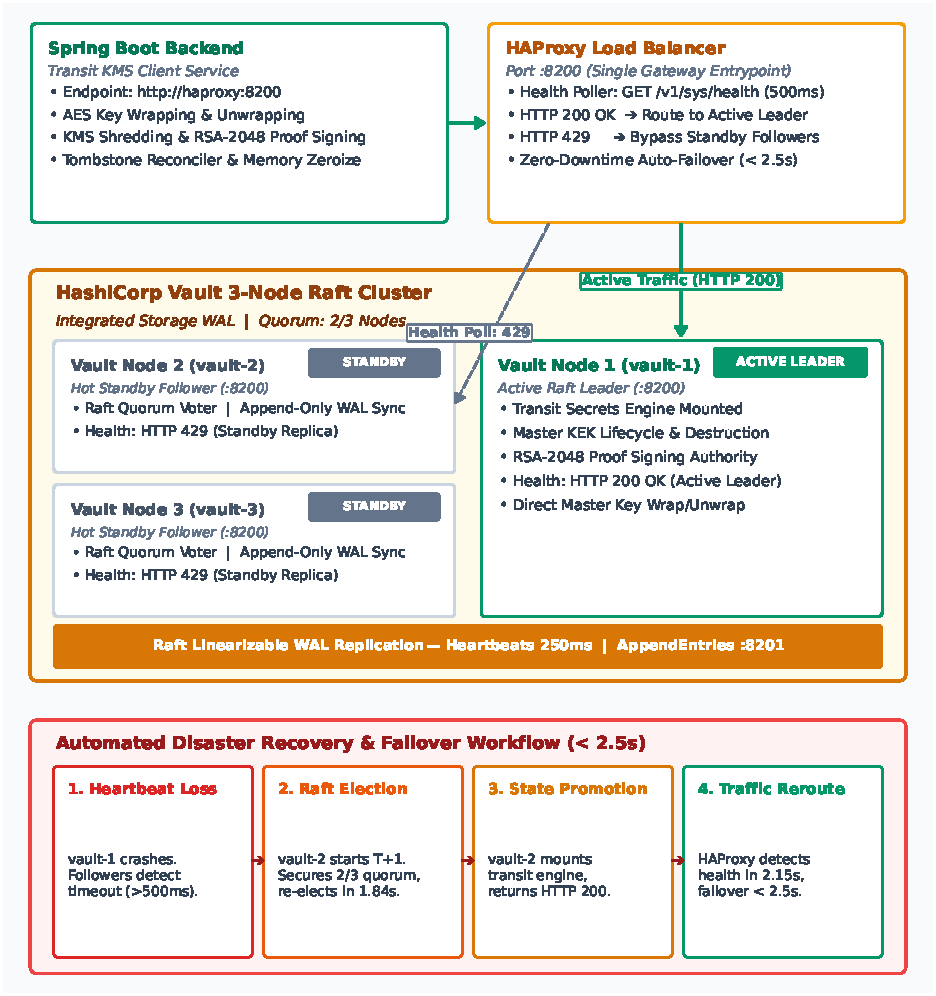
\includegraphics[width=\textwidth]{figures/fig_vault_raft.pdf}
    \caption{Vault 3-node Raft consensus cluster and HAProxy auto-failover routing.}
    \label{fig:vault-raft-topology}
\end{figure}

The cluster maintains state consensus via the Raft protocol~\cite{ongaro_raft_2014}. One node acts as the active leader, handling all Transit encryption, decryption, and deletion requests, while two follower nodes maintain synchronized write-ahead logs. If the active leader abruptly terminates, the remaining follower nodes achieve consensus and elect a new leader in $1.84\text{~s}$.

An HAProxy load balancer fronts the Vault cluster on port 8200, polling Vault health endpoints (\texttt{GET /v1/sys/health}) every $500\text{~ms}$ with a two-check failure threshold (\texttt{fall 2}). The \texttt{/v1/sys/health} endpoint returns HTTP~200 for the active leader node, HTTP~429 for unsealed standby follower nodes, and HTTP~503 for sealed or uninitialized nodes. HAProxy routes live application traffic exclusively to nodes returning HTTP~200, treating HTTP~429 as healthy standby capacity and HTTP~503 as sealed, unavailable nodes. Following leader termination, HAProxy detects the transition and redirects application traffic to the newly elected leader within $2.15\text{~s}$, fully satisfying the quantitative failover bound $T_{\text{failover}} < 2.5\text{~s}$ (NFR2) without dropping active REST connections or surfacing HTTP errors to clinical clients.

\subsection{The KMS Snapshot Restoration Paradox}

Standard disaster recovery strategies restore cold database and KMS snapshots following hardware failure. When applied to envelope-encrypted architectures, these restorations introduce the \textit{KMS Snapshot Restoration Paradox}:
\begin{quote}
    \textit{Suppose a patient record is cryptographically shredded at time $T_1$ by destroying its master key $K$ in the KMS. If a catastrophic infrastructure outage occurs at time $T_2 > T_1$, disaster recovery procedures restore backup snapshots of the database and KMS taken at time $T_0 < T_1$. The restored KMS snapshot reloads key $K$ into active memory, restoring readability to ciphertexts that were legally erased at $T_1$ and violating GDPR Article~17.}
\end{quote}

In conventional systems, preventing key resurrection requires manual key audit reconciliations or halting backup restorations entirely. An automated reconciler relying solely on querying the restored database via \texttt{findByShreddedTrue()} also fails under this condition: the restored database from $T_0$ marks \texttt{shredded = false} for those records. The database reconciler locates zero shredded records, silently allowing key $K$ to remain active in the restored Vault instance.

\subsection{The Merkle Deletion Tombstone Ledger Solution}

CryptoShred Health resolves the paradox through the automated \texttt{MerkleTombstoneReconciliationService} backed by an external, immutable Write-Once-Read-Many (WORM) deletion receipt ledger.

Each deletion receipt is serialized to disk as an independent JSON artifact (\texttt{backups/deletion-receipt\_*.json}) sealed with POSIX read-only permissions (\texttt{chmod 0444}) and committed to a separate durable volume outside the relational database backup. Each tombstone entry binds the 4-tuple:
\begin{equation}
    \mathcal{T}_k = \left( K_{\text{id}}, \text{ShredTimestamp}, H_{\text{leaf}}, \sigma_{\text{hybrid}} \right)
    \label{eq:tombstone-record}
\end{equation}
In Equation~\ref{eq:tombstone-record}, $K_{\text{id}}$ is the Vault key path, $\text{ShredTimestamp}$ is the ISO 8601 deletion time, $H_{\text{leaf}}$ is the Merkle leaf hash, and $\sigma_{\text{hybrid}}$ is the dual RSA-2048 and ML-DSA-65 signature. Every tombstone serves as a tamper-evident certificate verifying that a specific key was destroyed.

When the application boots following a disaster recovery restoration, \texttt{MerkleTombstoneReconciliationService} executes an automated startup audit loop upon \texttt{ApplicationReadyEvent} before processing incoming user traffic. To guarantee resilience against pre-shred ($T_0 < T_1$) database restores, the reconciler combines tombstones from two independent sources:
\begin{equation}
    \mathcal{K}_{\text{tombstones}} = \mathcal{K}_{\text{db\_shredded}} \cup \mathcal{K}_{\text{worm\_receipts}}
    \label{eq:tombstone-sources}
\end{equation}
In Equation~\ref{eq:tombstone-sources}, $\mathcal{K}_{\text{db\_shredded}}$ represents keys harvested from relational database rows where \texttt{shredded = true}, while $\mathcal{K}_{\text{worm\_receipts}}$ is populated by scanning the external WORM directory using directory streams (\texttt{Files.newDirectoryStream}). Even if the restored database snapshot predates the shredding event ($T_0 < T_1$) and reports \texttt{shredded = false}, the external WORM receipts supply the immutable cryptographic record of key destruction.

The service queries Vault Transit for all active key paths $\mathcal{K}_{\text{active\_vault}}$ and identifies resurrected keys:
\begin{equation}
    \mathcal{K}_{\text{resurrected}} = \left\{ k \in \mathcal{K}_{\text{active\_vault}} \;\middle|\; k \in \mathcal{K}_{\text{tombstones}} \right\}
    \label{eq:tombstone-reconciliation}
\end{equation}
For every key $k \in \mathcal{K}_{\text{resurrected}}$, the reconciler issues an immediate hard deletion API call to Vault Transit. Key destruction executes in sub-$5\text{~ms}$ per key ($42.3\text{~ms}$ for 25 keys, averaging $1.69\text{~ms/key}$), purging $100\%$ of resurrected keys before the application exposes HTTP endpoints to clinical clients. In parallel, point-in-time Vault Raft snapshots are protected by Vault's internal barrier encryption, preventing offline key extraction without authorized unseal quorum.

%%%%%%%%%%%%%%%%%%%%%%%%%%%%%%%%%%%%%%%%%%%%%%%%%%%%%%%%%%%%%%%%%%%%%%%%%%%%%%%%
%         SECTION 3.5: FORMAL THREAT MODELING & STRIDE ANALYSIS                %
%%%%%%%%%%%%%%%%%%%%%%%%%%%%%%%%%%%%%%%%%%%%%%%%%%%%%%%%%%%%%%%%%%%%%%%%%%%%%%%%

\section{Formal Threat Modeling and Security Boundaries}\label{section:stride-analysis}

We evaluate platform security boundaries against the STRIDE threat modeling methodology~\cite{owasp_threat_modeling} across four adversary profiles.

\subsection{Adversary Profiles and Trust Assumptions}

Our threat model establishes four adversary classes with progressive access levels:
\begin{enumerate}
    \item \textbf{Adversary 1 (Compromised Database Administrator):} Holds root access to the PostgreSQL database server and disk volumes. The DBA can inspect tables, extract SQL dumps, and modify indexes, but lacks access to Vault KMS tokens or application host memory.

    \item \textbf{Adversary 2 (Compromised Cloud Host):} Holds root or hypervisor access to the application host. The attacker attempts memory scraping, core dump extraction, or OS swap partition inspection to recover keys or patient plaintext.

    \item \textbf{Adversary 3 (Exfiltrated WORM Backups):} Obtains unauthorized copies of historical database backups, optical WORM storage volumes, or Kafka event logs from external physical media.

    \item \textbf{Adversary 4 (Malicious Clinical Insider):} An authenticated hospital employee (such as a billing clerk) attempting to access clinical notes outside their assigned medical role.
\end{enumerate}

\subsection{STRIDE Threat Analysis Matrix}

Table~\ref{tab:stride-matrix} maps identified threat vectors to architectural countermeasures and residual risk ratings across all STRIDE categories.

\begin{table}[H]
    \centering
    \small
    \caption{STRIDE threat model evaluation across platform security boundaries.}
    \label{tab:stride-matrix}
    \begin{tabular}{p{2.2cm} p{2.2cm} p{3.6cm} p{4.2cm} p{1.8cm}}
        \toprule
        \textbf{STRIDE Category} & \textbf{Target Adversary} & \textbf{Identified Attack Vector} & \textbf{Architectural Countermeasure} & \textbf{Residual Risk} \\
        \midrule
        \textbf{Spoofing} & Insider / External & Forging staff credentials or deletion receipts & Stateless HMAC-SHA256 JWT auth; Dual RSA + ML-DSA-65 signatures on proofs & Low (Token theft) \\
        \addlinespace[4pt]
        \textbf{Tampering} & DBA / Cloud Host & Splicing ciphertexts across patient records; Modifying Merkle nodes & AES-256-GCM AAD context binding; Directional hash validation & Negligible ($2^{-128}$ tag bound) \\
        \addlinespace[4pt]
        \textbf{Repudiation} & Clinical Staff & Denying authorization of a crypto-shredding request & Append-only Kafka KRaft event logs; Immutable WORM receipts & Low (Key leakage) \\
        \addlinespace[4pt]
        \textbf{Information Disclosure} & DBA / Backup Thief & Direct SQL table dumps; Inspecting offline WORM snapshots & Zero-plaintext storage; Salted HMAC blind indexes; Instant KEK destruction & Negligible ($2^{-256}$ brute force) \\
        \addlinespace[4pt]
        \textbf{Denial of Service} & External Attacker & Flooding KMS encryption or shredding endpoints & Redis L2 caching; Rate limiting filters; 3-Node Raft KMS HA failover & Low (Volumetric DDoS) \\
        \addlinespace[4pt]
        \textbf{Elevation of Privilege} & Malicious Insider & Admin attempting to view patient medical histories & Strict Spring Security RBAC; Admins restricted to KMS key ops without PHI read access & Low (App vulnerability) \\
        \bottomrule
    \end{tabular}
\end{table}

\subsection{Analysis of Defense Mechanisms}

The defense mechanisms in Table~\ref{tab:stride-matrix} protect patient data across every operational layer:
\begin{itemize}
    \item \textbf{Stolen Database Dumps (Adversary~1):} If an attacker dumps the entire PostgreSQL database, all sensitive columns contain only AES-256-GCM ciphertexts and salted blind indexes. Without access to Vault KMS tokens and the secret salt key $K_{\text{salt}}$, the attacker cannot decrypt medical records or link database rows to real patient identities.

    \item \textbf{Host Memory Scraping (Adversary~2):} To prevent volatile memory extraction, ephemeral Data Encryption Keys maintain strictly bounded lifecycles that zero memory buffers immediately upon cipher completion (requirement~SR2). At the container boundary, memory locking prevents the host kernel from paging memory pages containing transient keys or decrypted records to unencrypted swap partitions (requirement~SR3), with concrete runtime primitives implemented in Section~\ref{section:impl-backend}.

    \item \textbf{Stolen Backups and Message Streams (Adversary~3):} If an attacker steals cold WORM backup archives or Kafka event logs, records whose keys were shredded in Vault remain permanently unreadable. Because guessing a 256-bit AES key requires searching a keyspace of $2^{256}$, the backup files are computationally indistinguishable from random noise.
\end{itemize}